\section{Watermark Overview}
Watermarking involves modifying a piece of content to include a message related to that content. The origins of watermarking can be traced back to medieval times, evolving alongside advancements in papermaking and the growing need for document authentication and security. The practice first emerged in 13th century Italy, where papermakers integrated basic designs or symbols into paper molds, resulting in subtle variations in thickness. When held up to light, these watermarks became visible, functioning as identification for the papermaker or as an indicator of quality. Watermarking involves modifying a piece of content to include a message related to that content. The origins of watermarking can be traced back to medieval times, evolving alongside advancements in papermaking and the growing need for document authentication and security. The practice first emerged in 13th century Italy, where papermakers integrated basic designs or symbols into paper molds, resulting in subtle variations in thickness. When held up to light, these watermarks became visible, functioning as identification for the papermaker or as an indicator of quality.

By the 18th century, watermarks began incorporating more elaborate designs and patterns, often reflecting the brand of the paper manufacturer or adding an artistic touch. This period marked a shift from purely utilitarian watermarks to those with aesthetic appeal. In the early 20th century, the advent of digital technology led to the transformation of traditional paper watermarks into digital counterparts. In the realm of digital media, these digital watermarks serve diverse purposes, including safeguarding copyright, authenticating content, and facilitating tracking. They are imperceptible to the human eye and became prevalent in the late 20th century, embedded within digital files such as images or documents. Nowadays, watermarks continue to fulfill essential roles in security, branding, and authentication across physical and digital domains, adapting to the evolving needs of industries and technologies.

Paper watermarks first appeared in Italy in 1282, over a thousand year since papermaking had been invented in China. The marks were made by adding thin wire patterns to the paper molds. The earliest watermarks were used for practical functions such as identifying the molds on which sheets of papers were made, or as trademarks for ownership, or they might just represent mystical signs or serve as decoration. By the eighteenth century, they have been used in Europe and America for precise purposes, trademarks and manufacturing records. It was also the first time watermarks were used as anticounterfeiting measures on money and other documents. From that time, watermark embedding systems and watermark attacking systems prompted advances for each other, as a subbranch of security and steganography.

\subsection{Watermark Embedding}
In general, watermarks can be as simple as an extra logotype or text added to an image that are subtle with human visual system, or an imperceptible signal embedded to an original signal. Subsequently, watermarks can be broadly classified into two primary categories - visible and invisible.

Visible watermarks are intentionally noticeable and easily seen by the human eye. Typically overlaid onto the surface of an image or document, they often consist of logos, text, or symbols. The principal aim of visible watermarks is to identify the origin or ownership of the content and deter unauthorized use. While effective in conveying ownership, visible watermarks may occasionally impact the aesthetic appeal of the content.

On the other hand, invisible watermarks are like secret codes you cannot see right away. They get mixed into the picture using digital tricks, such as adding noise or embedding unique code within the pixels of a digital image without changing how it looks. Invisible watermarks do different jobs, like protecting copyrights, proving if something is real, or keeping track of things. They are useful for digital stuff, like pictures or documents, because you do not see any changes on the outside. To find invisible watermarks, you need special computer programs or smart processes that can uncover the hidden information.

In our project, we are focusing on those watermarks that catch your eye—the visible ones. They mess with the image when they are added, and that is the puzzle we are tackling. We are figuring out how to use a diffusion-based method to bring back the original image after we have wiped out those noticeable watermarks, like totally removing them from the picture.

We now then work on putting the watermark into images. The aim is to enhance the image's privacy, adding an extra layer of security. The introduction of a watermark provides a level of protection for the image. Watermarks come in various types, such as those made of text or images. In our project, we are specifically concentrating on image watermarks. Our objective is to embed the image watermark into the original image, making it challenging to identify or detect compared to text watermarks, which are somewhat easier to recognize. Subsequently, we plan to examine and remove these watermarks through detection methods.

There are various methods to incorporate a watermark into an image. Tao et al. \cite{tao2014robust} have researched some methods to embed a robust watermark, ranging from random embedding to intentional placement. In intentional embedding, the watermark can alter the image's appearance, making it challenging for humans to observe or confusing for classifier models, leading to incorrect predictions. In our approach, we choose to randomly embed the watermark within the image, in which details will be discussed in Chapter \ref{chap:experiment}. This section will delve into the specifics of our method for watermark embedding.


In general, watermarks can be as simple as an extra logotype or text added to an image that are subtle with human visual system, or an imperceptible signal embedded to an original signal. Those in the former case are conventionally called visible watermarks, where diffusion models can be applied to transform a watermarked region or the whole image into a realistic unwatermarked version. Those in the latter case are called invisible watermarks with two broad groups of generating models - \textit{communication-based} models and \textit{geometric models} \cite{cox2007digital}. We focus on visible watermarks only. A visible watermark embedding algorithm should satisfy some requirements, such as

\begin{enumerate}
    \item The watermark is perceptible in both gray and colored images.
    \item The watermark should be perceptible in pixels with different characteristics: texture, plain and edge.
    \item The watermark should not be too obtrusive.
    \item The watermark should be robust against several common attacks.
    \item Watermark embedding process should be automatic for kinds of images.
\end{enumerate}

An image can be represented a three-channel two-dimensional array. Compressed into the gray scale, each pixel takes integer values in the interval $[0,256]$.  The following watermark embedding model for binary watermark \cite{yu2013new} is based on the observation that the ability of human eyes to distinguish between two close pixel values tend to be highest in the interval $[64,128]$, i.e. for a pixel $p\in [64,128]$, a human may be able to distinguish between $p$ and $p+1$. Denote by $y$ this minimal perceptible difference. They approximate the relation as
\begin{equation}
    y=\begin{cases}
        -\dfrac{1}{8}p+6,             & \text{ if } p\in [0, 32]   \\
        -\dfrac{1}{32}p+3,            & \text{ if } p\in [33, 64]  \\
        -\dfrac{1}{96}p+\dfrac{1}{3}, & \text{ if } p\in [65, 255] \\
    \end{cases}
\end{equation}

\begin{figure}
    \centering
    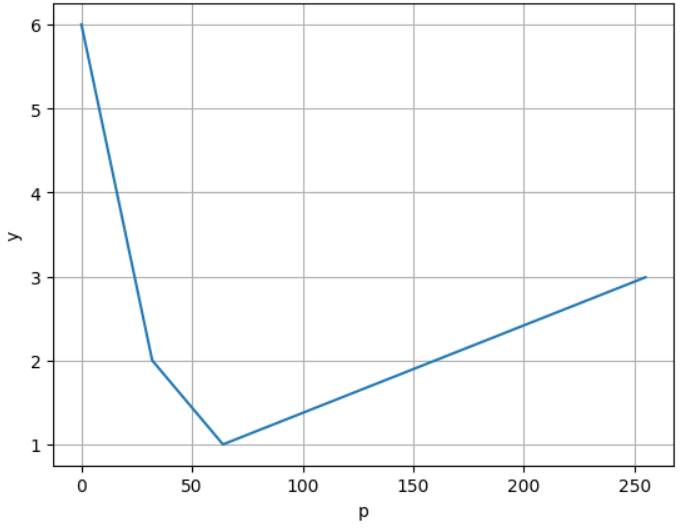
\includegraphics[width=0.5\linewidth]{img/resolution.png}
    \vspace{0.5cm}
    \caption{The approximation of human eye resolution on the gray scale}
    \label{figure:human-eye-resolution}
\end{figure}

Therefore, the difference between a clean pixel and a watermarked pixel must obey this human distinguishing ability. The watermark strength $\alpha$ depending on the pixel value is given by
\begin{equation}
    \alpha(p)=cy(p),
\end{equation}
where $c$ is a constant hyperparameter. The watermarked image is obtained pixel-by-pixel by
\begin{equation}
    p'(i,j)=p(i,j)+\alpha
    (p(i,j))w(i,j),
\end{equation}
where
\begin{itemize}
    \item $p(i,j)$ is the original pixel
    \item $w(i,j)\in\{0,1\}$ is the watermark value
\end{itemize}

The embedding process is applied for each channel and finally combined to a single watermarked image.

\subsection{Watermark Removal}
% intro with surveys
Digital watermarks are frequently employed for copyright identification in images, preventing unauthorized use of online images. Additionally, techniques for attacking watermarks aim to effectively eliminate watermarks from host images. The strength of a watermark against such attacks is crucial for safeguarding image copyrights. Methods for removing watermarks have been investigated to assess and enhance the durability of watermarks. In this section, we will explore existing methods and discuss our approach to watermark removal.

Oldest methods for getting rid of watermarks usually require users to point out where the watermark is located, and then they use special features to remove it, such as Independent Component Analysis \cite{pei2006novel} or Color Space Transformation \cite{park2012identigram}. Also, some methods make use of multiple images \cite{dekel2017effectiveness} \cite{gandelsman2019double}. But, these methods need a lot of information ahead of time, and they only work well on a limited number of examples.

\begin{figure}[H]
    \centering
    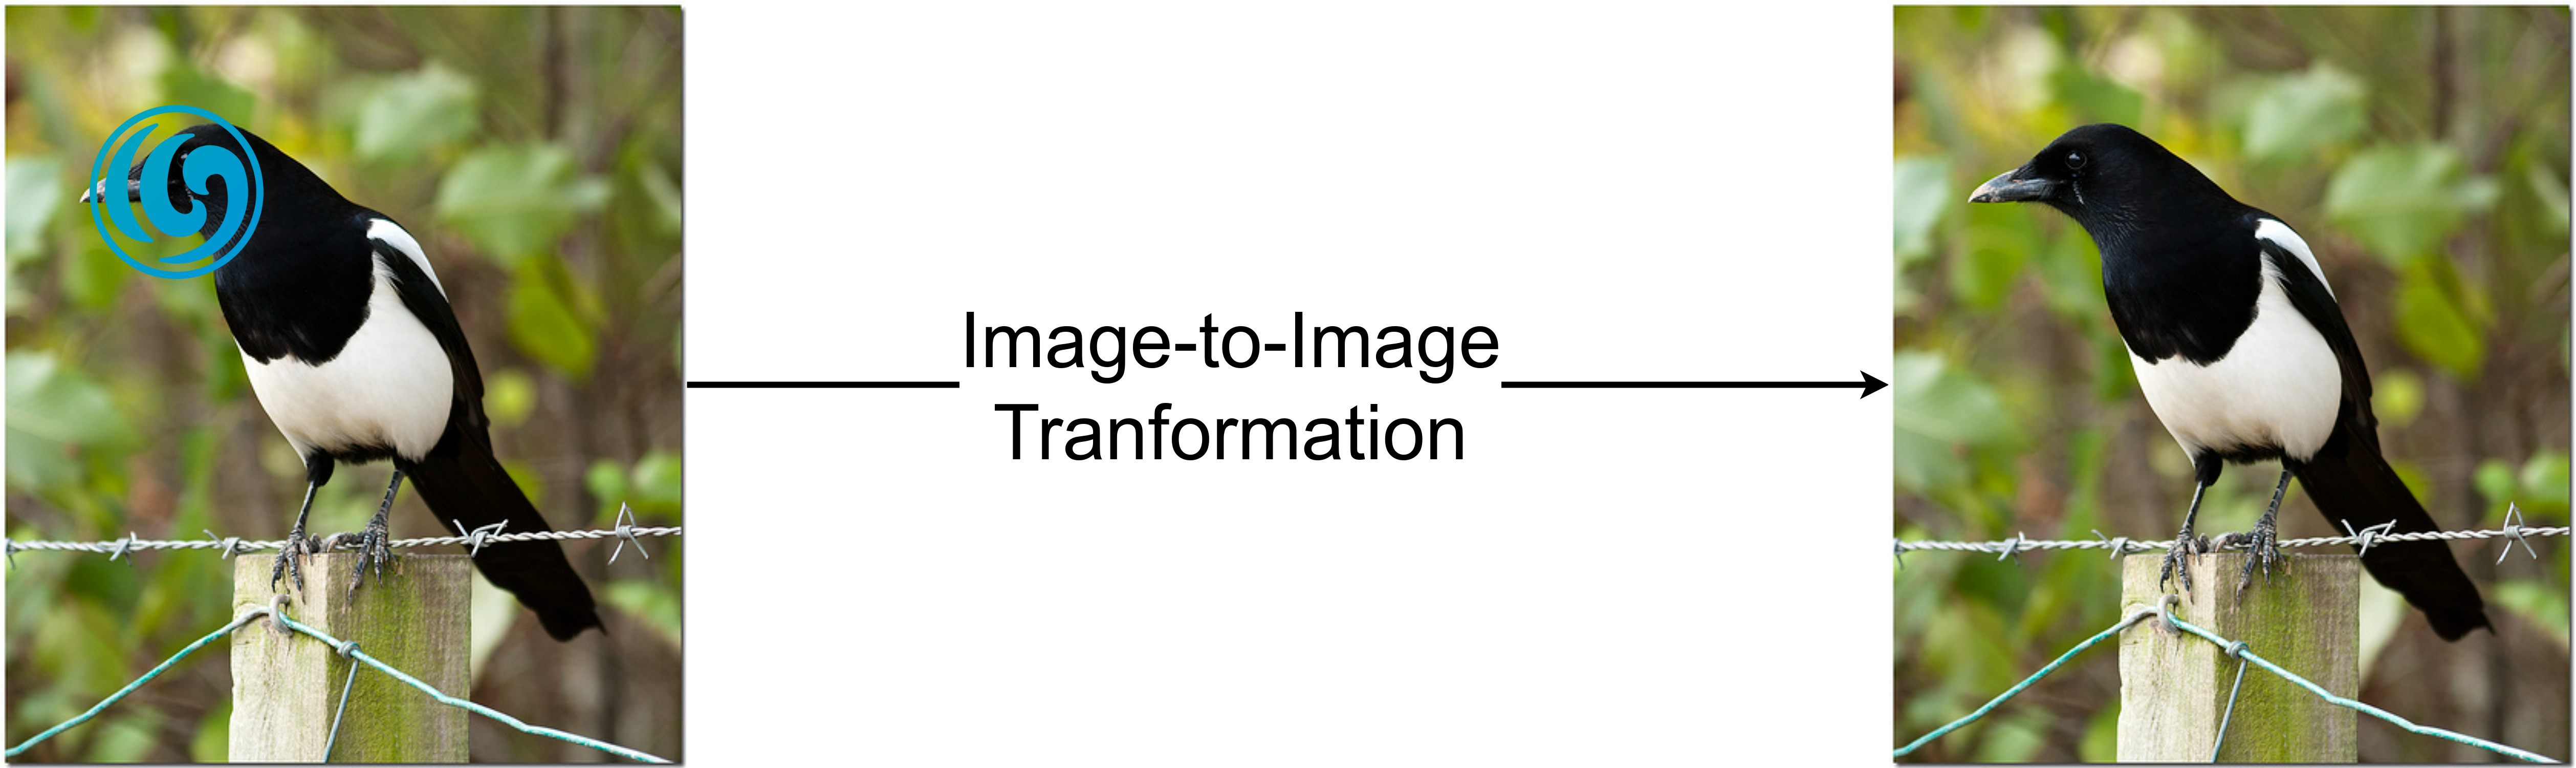
\includegraphics[width=0.75\linewidth]{img/watermark_removal_1.png}
    \caption{Watermark Removal with Image-to-Image methods}
    \label{figure:img2img1}
\end{figure}

More recently, deep learning-based methods show great power in many computer vision tasks \cite{he2016deep}, and this approach has been applied to remove visible watermarks too \cite{li2019towards} \cite{cheng2018large}  \cite{hertz2019blind}. But, before using these methods, you need a detection model that can already identify watermarks \cite{cheng2018large}, or they only focus on getting rid of the watermark without thinking about the whole image as an Image-to-Image Translation problem \cite{li2019towards}, as generally illustrated in Figure \ref{figure:img2img1}. Plus, the datasets they often use only have gray-scale watermarks. Nowadays, though, most watermarks are in color. Recently, a method was designed to find, erase, and fix the motif in just one go \cite{hertz2019blind}. However, these methods do not pay much attention to learning about the damaged part of the image.

% \textcolor{red}{CNN version (U-Net): https://arxiv.org/pdf/2403.05807.pdf}
% \textcolor{red}{Note about one-stage watermark removal}
% \subsection{Image-to-Image methods}
% Summary some methods in Image-to-Image
